\chapter{Conclusions}
The proposal describes methods for designing VPNs, while much emphasis is
placed upon the use of structured overlays, much of what described can be used
generically.  The contributions so far describe a scalable, self-configuring,
decentralized VPNs supported by a structured overlay.  Completed components of
this work include:
\begin{itemize}
\item \textbf{Relays} - to enable two-hop connections between peers that cannot
form direct connections.
\item \textbf{Private Virtual Overlays} - secure, self-configuring overlay as
the basis for a structured overlay VPN.
\item \textbf{Group environments} - User-friendly environments to generate
files to ease configuration of complex systems.
\item \textbf{Local VPN configuration} - VPN architect supporting Interface,
Router, and a novel Hybrid mode for various environments.
\end{itemize}

The remaining components of my work are overlay-aware TCP, userspace
(socket-based) VPN, and improving structured P2P VPNs through different usage
patterns.  For each of these tasks, I will design, implement, and evaluate the
approaches.  The results will lead to new interesting designs of VPNs using
structured overlays.  A schedule for my work is shown in Figure~\ref{fig:gantt}.

\begin{figure}[ht]
\centering
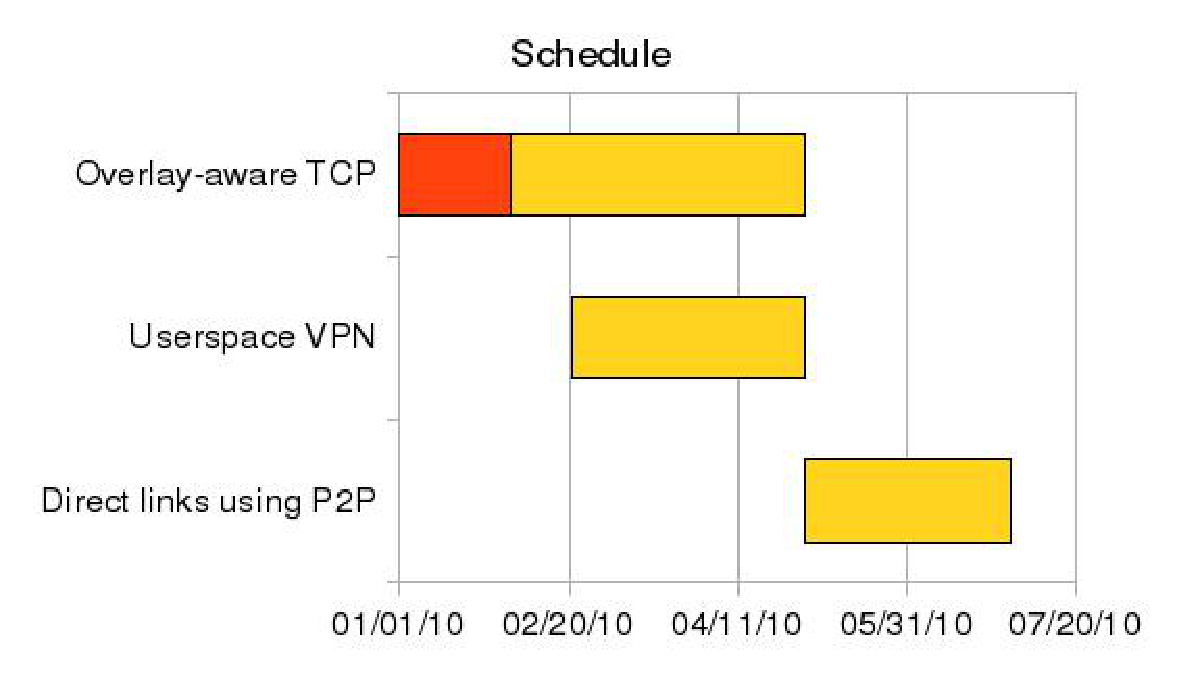
\epsfig{file=figs/schedule.eps, width=4in}
\caption{Schedule for my proposed work.}
\label{fig:latency}
\end{figure}
